%!TEX root =  main.tex
\section{Performance evaluation}
\label{sec:experiments}


In this section, we present the results found for \appname\ with
different loads and partitionings and compare them with
\ssmr{}~\cite{bezerra2014ssmr} and \dssmr.  In
Section~\ref{sec:evaluation:setup}, we describe the environment where
we conducted our experiments.  In
Section~\ref{sec:evaluation:methodology}, we describe how we designed
the experiments and our methodology.  In
Section~\ref{sec:evaluation:results}, we show the results.

\subsection{Environment and configuration parameters}
\label{sec:evaluation:setup}

We conducted all experiments on a cluster with two types of nodes: (a)
HP SE1102 nodes, equipped with two Intel Xeon L5420 processors running
at 2.5 GHz and with 8 GB of main memory, and (b) Dell SC1435 nodes,
equipped with two AMD Opteron 2212 processors running at 2.0 GHz and
with 4 GB of main memory. The HP nodes were connected to an HP
ProCurve 2920-48G gigabit network switch, and the Dell nodes were
connected to another, identical switch. Those switches were
interconnected by a 20 Gbps link.  All nodes ran CentOS Linux 7.1 with
kernel 3.10 and had the OpenJDK Runtime Environment~8 with the
\mbox{64-Bit} Server VM (build 25.45-b02).

We used the Holme-Kim model \cite{holme-kim} to generate all social graphs.
We created power-law graphs (also known as scale-free graphs) with a clustering coefficient varying from 0.6 to 1, 
this is the probability of whenever an edge $(v, w)$ is added to the graph, $v$ connects to some neighbour of $w$, 
In the experiments, we tested graphs with 10000 users with a varying percentage of edge-cuts (i.e., edges connecting vertices in different partitions).

\subsection{Methodology and goals}
\label{sec:evaluation:methodology}

In the experiments with our social network service, we focus on post
commands only since getTimeline commands are all single-partition.
Posts are more difficult to handle since the rate between
single-partition and multi-partition commands depends on the geometry
of the social graph and the technique used to partition the data.

When designing the experiments, we strived to answer the following questions.
\begin{itemize}
\item \emph{How does \dynastar compare to other approaches?} 
\item \emph{How does the number of partitions affect the performance of posts for a fixed social graph?}
\item \emph{How does \dynastar perform under dynamic workloads?}
\item \emph{When will the oracle become a bottleneck?}
\end{itemize}

We answer these questions for social graphs with different geometries
and using deployments with different number of partitions, with 2, 4
and 8 partitions.  We characterize a social graph using the percentage
of edge-cuts computed by METIS on a static graph, and use graphs with
0\%, 1\%, 5\% and 10\% of edge cuts.


\subsection{\dynastar vs. alternative systems}
\label{sec:evaluation:results}

As we see in Figure~\ref{fig:varying_edge_cut}, all the techniques
perform similarly on tests with strong locality, that is expected
because there are no cross-partition commands after the graph is
perfectly partitioned and no more moves occur in \dynastar or \dssmr,
also no synchronization among partitions is necessary for \ssmr.  As
the number of edge-cuts get higher however, \dssmr\ performance
decreases significantly.  This happens because with weak locality,
objects in \dssmr\ are constantly being moved back and forth between
partitions, and hardly converge in a stable configuration, the problem
only gets worse when the number of edge-cuts increases, as the number
of moves increases proportionally.  For \dynastar and \ssmr with a
static partitioning, we can see that the throughput scales with the
number of partitions, this is expected for both methods, up to a point
that the number of moves and cross-partition commands have a
considerable overhead in the execution.

\begin{figure*}[ht!]
	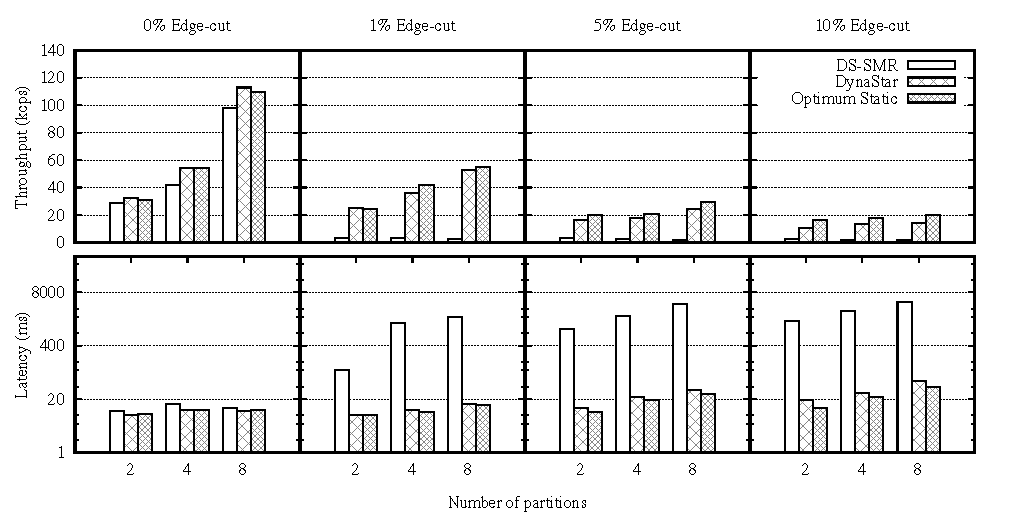
\includegraphics{figures/experiments/throughput-latency-avg-all}
	\caption{Throughput and latency, varying edge-cuts for different partitioning size}
	\label{fig:varying_edge_cut}
\end{figure*}


\subsection{Performance with the number of partitions}
\label{sec:evaluation:results}

\begin{figure}[ht]
	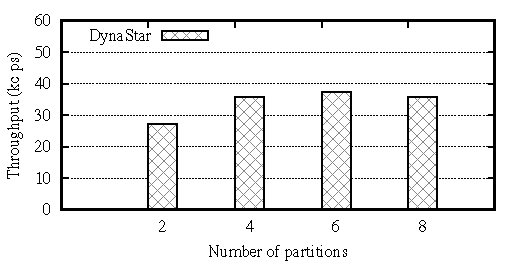
\includegraphics{figures/experiments/throughput-avg-vary-partition}
	\caption{Same graph in different partitioning}
	\label{fig:4p1p_varying_partition_size}
\end{figure}

\rjs{TODO(rjs): write this.}

\subsection{Performance under dynamic workloads}

Figure~\ref{fig:dynamic_load_tput} depicts dynamically repartitioning
on-the-fly.  We started the system with an empty graph. Then clients
continuously create users and links between them during the experiment
(running the follow command).  The oracle monitors changes in the
graph's structure and trigger a repartitioning when the number of
changes exceed a threshold.  Each time the repartitioning took place,
the partitioning became better, that helps the throughput increase.

\begin{figure}[ht]
	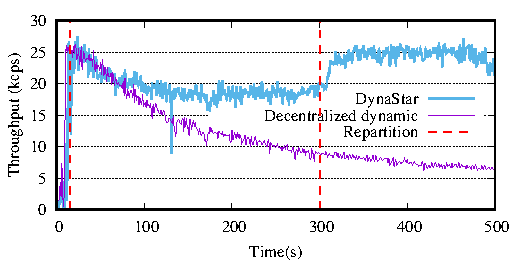
\includegraphics{figures/experiments/dynamicload-tp-move-4p}
	\caption{Adding nodes and repartitioning dynamically}
	\label{fig:dynamic_load_tput}
\end{figure}



\subsection{The performance of the oracle}

METIS performs well in graphs with less than 10 million nodes, and
scales linearly as seen in Figure~\ref{fig:metis_size_time}, with both
memory and cpu usage.

\begin{figure}[ht!]
  \centering
    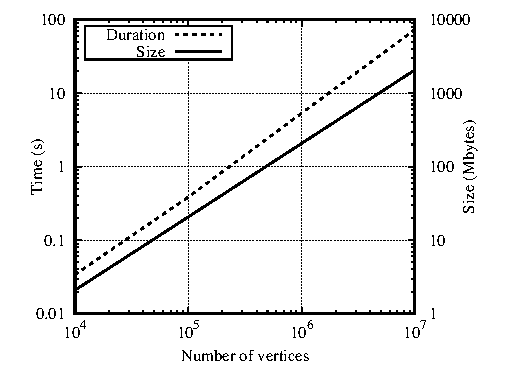
\includegraphics[width=\columnwidth]{figures/metis_size_time}
	\caption{METIS processor and memory usage}
	\label{fig:metis_size_time}
\end{figure}

To test if the oracle can be a bottleneck, in
Figure~\ref{fig:cpu_oracle} we show the average load over time in the
oracle.  The load is higher in the beginning, when the clients did not
yet cache the requests, but diminish over time. Access to the oracle
is necessary only when clients have an invalid log or when a
repartition happens.

\begin{figure}[ht]
	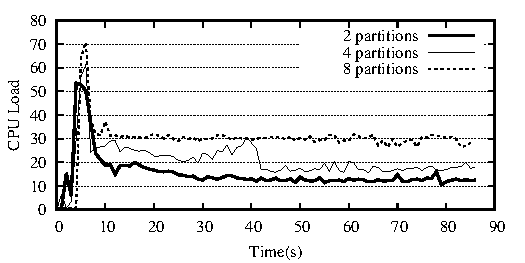
\includegraphics{figures/experiments/oracle-load}
	\caption{CPU load in the oracle}
	\label{fig:cpu_oracle}
\end{figure}

\label{sec:evaluation:strongloc}

